\section{Concepts}
\label{g1:sec:concepts} % TODO Adopt group prefix

As mentioned in the introduction the goal is to connect two seperate systems to have another HMI. Instead of a mice and keyboard 

\subsection{Polypheny}
"The last years have seen a vast diversification on the database market. In contrast to the “one-size-fits-all” paradigm according to which systems have been designed in the past, today’s database management systems (DBMS) are tuned for particular workloads. This has led to DBMSs optimized for high performance, high throughput read / write workloads in online transaction processing (OLTP) and systems optimized for complex analytical queries (OLAP). However, this approach reaches a limit when systems have to deal with mixed workloads that are neither pure OLAP nor pure OLTP workloads. In such cases, multistores are increasingly gaining popularity. Rather than supporting one single database paradigm and addressing one particular workload, multistores encompass several DBMSs that store data in different schemas and allow to route requests on a per-query level to the most appropriate system. In this paper, we introduce the multistore ICARUS . In our evaluation based on a workload that combines OLTP and OLAP elements, we show that ICARUS is able to speed-up queries up to a factor of three by properly routing queries to the best underlying DBMS." - Quote from Icarus: Towards a Multistore Database System
\newline
\\
Polypheny addresses exactly this problem. For our project we are not really dependant on the polystore aspect of the database but on the relational algebra part. Polypheny supports a graphical user interface where SQL queries can be built and connected via drag an drop and ran afterwards. Since the user must understand SQL or relational algebra to build such a tree, our implementation also does not address users which can not build statements.

\subsection{Deepmime}
Deepmime is a gesture recognition implementation based on a 3D residual neural network (ResNet). A residual neural network is an artificial neural network (ANN) of a kind that builds on constructs known from pyramidal cells in the cerebral cortex.\footnote{\url{https://en.wikipedia.org/wiki/Residual_neural_network}} For the implementation to recognise gestures on the fly, the skip connection is the relevant aspect for choosing a ResNet. The implementation we worked with takes a pre-trained model and classifies the video feed into a probability which labels it could be. 

\subsection{Human-Machine Interaction}

\subsection{Architecture}
\begin{figure}[H]
    \centering
    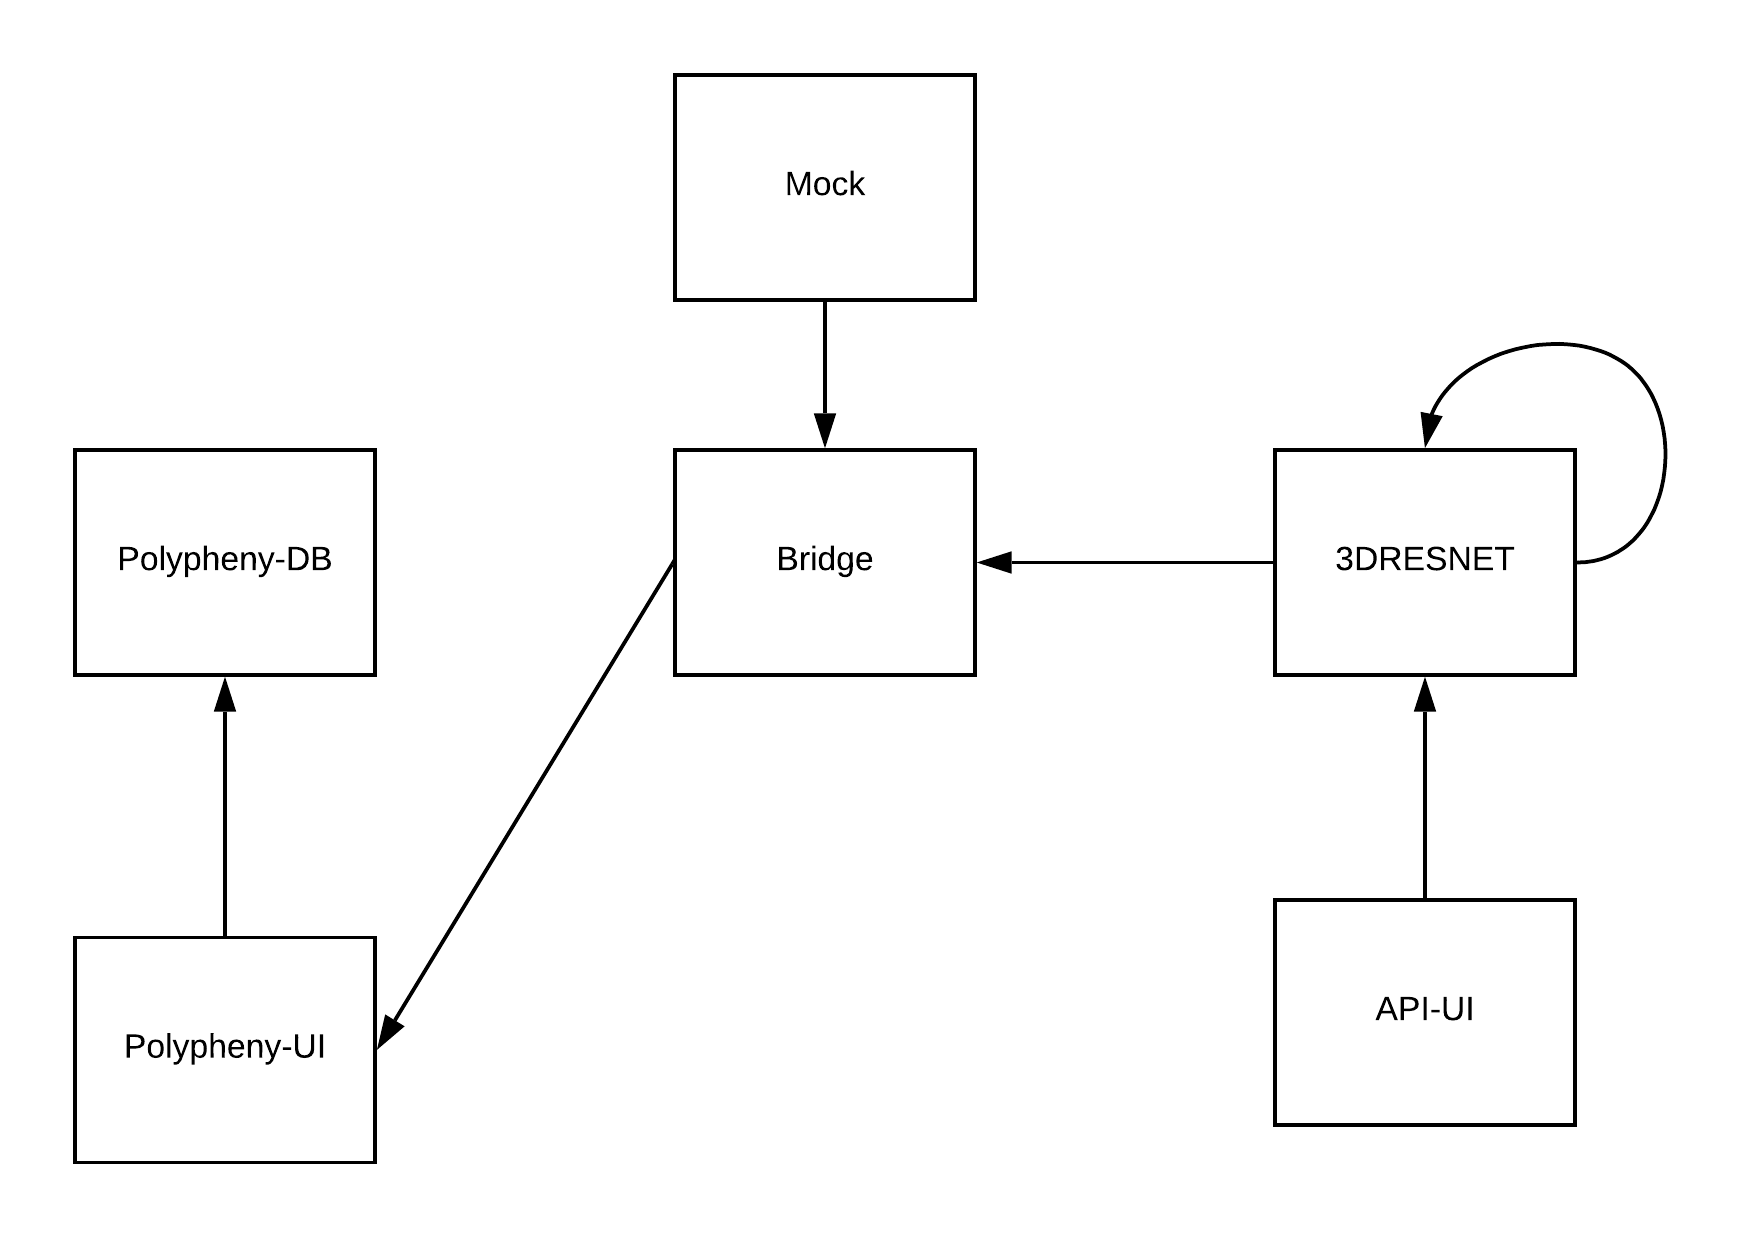
\includegraphics{reportContent/images/architecture.png}
    \caption{Architecture Diagram}
    \label{fig:my_label}
\end{figure}{}

\\
\\
\\
Polypheny - Polystore - Database - Relational Algebra as graphical interface with nodes where a SQL statement can be built. 

Gesture Recognition - 3d resnet - Concept shown in Pattern Recognition

Own Json Parser

Every Node is represented as node class redone in Python 

Gesture gets detected - send to our server as string - parsed to the json tree - then send to polypheny and re arranged

